\documentclass[english, a4paper,12pt]{article}
\usepackage[a4paper, top=2cm, bottom=2cm,right=2cm,left=2cm]{geometry}
\date{} 
\usepackage[utf8]{vietnam}
\usepackage{textcomp, graphicx, titling, tkz-tab, changepage}
\usepackage{changepage, xcolor, amsmath, fancyvrb, minted, caption} 
\usepackage{booktabs}
\usepackage{tabularx}
\definecolor{LightGray}{gray}{0.95}

\usepackage[english]{babel}
\addto\captionsenglish{
  \renewcommand{\contentsname}
  {Table of Contents}
}

\begin{document}
\begin{titlepage}
\begin{center}
\textbf{UNIVERSITY OF INFORMATION TECHNOLOGY}

\textbf{FACULTY OF COMPUTER SCIENCE}

\vspace{1cm}

\vspace{1cm}

\textbf{SOLVING KNAPSACK PROBLEMS USING GOOGLE OR TOOLS}

\vspace{2cm}

\includegraphics[width= 5cm]{logo.png}
\vspace{2cm}

\textbf{Instructor: } Luong Ngoc Hoang

\vspace{0.5cm}

\textbf{Student:} Ha Huy Hoang - 22520460
\vspace{0.5cm}
\\
\textbf{Class:} CS106.O21
\vspace{2cm}
\tableofcontents
\end{center}
\end{titlepage}
\section*{1. Experiment set-up}
\addcontentsline{toc}{section}{1. Experiment set-up}
\hspace*{7mm}To set up the experiments, I first install the or-tools module and clone the directory containing the test-case set for the experiments. I follow the instructions from the homepage to implement a solver for Knapsack problems. Additionally, I need to retrieve all files from the repository and read and convert data from them. However, there are too many files in the repository, so for each group, I will take all different sizes and for each size, I will take 10 files (in both the R01000 and R10000 directories). In total, I have 13x8x10 files as test cases for this problem. I will set the time limit to 180 seconds (equivalent to 3 minutes). If the algorithm’s solution time touches or exceeds 180 seconds, it will be considered non-optimal according to the reference included in Google OR-Tools.
\begin{center}
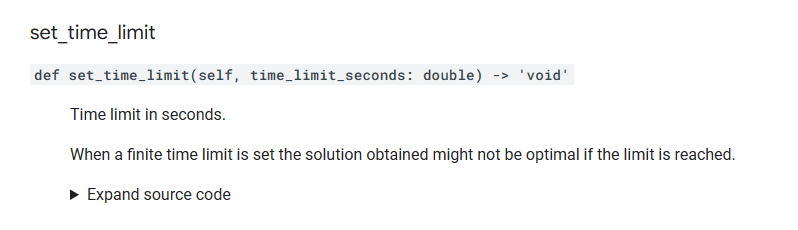
\includegraphics[width=10cm]{image.png}
\end{center}

\hspace*{7mm} In this experiment, I will have 3 files: 
\begin{itemize}
\item \textbf{solver.py}: used to clone data and run random test cases.
\item\textbf{random\_file\_result.py}: used to select 8 random result files in each group for easy statistics (1040 testcases will create almost 20 pages table).
\item 
\textbf{check\_optimal\_of\_test\_group.py}: used to evaluate the optimality rate of the result files for each test case group.
\end{itemize}


\section*{2. Statistics and Evaluation}
\addcontentsline{toc}{section}{2. Statistics and Evaluation}
\subsection*{2.1. Statistics}
\addcontentsline{toc}{subsection}{2.1. Statistics}
\hspace*{7mm}I have randomly selected 8 files from each test group to make the statistical analysis lighter.
\begin{itemize}
\item \textbf{Test case}: the path of file test case.
\item \textbf{Time}: duration of the algorithm’s execution in seconds.
\item \textbf{Value}:  total value of optimal packed items.
\item \textbf{Weight}: total weight of optimal packed items.
\item \textbf{Optimal}: True, if it is an optimal solution. False, if is a non-optimal solution.
\end{itemize}
 \begin{center}
 \small\begin{tabularx}{0.95\textwidth}{|>{\raggedright\arraybackslash}Xrrrr|}
\hline
\textbf{Test case} & \textbf{Time} & \textbf{Value} & \textbf{Weight} & \textbf{Optimal} \\
\hline
\addlinespace
\hline
00Uncorrelated \textbackslash n00100 \textbackslash R01000 \textbackslash s025.kp & 0.000 & 37308 & 24402 & True \\
00Uncorrelated \textbackslash n00100 \textbackslash R10000 \textbackslash s056.kp & 0.000 & 358851 & 243958 & True \\
00Uncorrelated \textbackslash n00050 \textbackslash R01000 \textbackslash s083.kp & 0.000 & 19444 & 10766 & True \\
00Uncorrelated \textbackslash n00050 \textbackslash R10000 \textbackslash s091.kp & 0.000 & 213998 & 135467 & True \\
00Uncorrelated \textbackslash n05000 \textbackslash R01000 \textbackslash s060.kp & 0.000 & 2006371 & 1250925 & True \\
00Uncorrelated \textbackslash n05000 \textbackslash R10000 \textbackslash s090.kp & 0.000 & 20368880 & 12412821 & True \\
00Uncorrelated \textbackslash n02000 \textbackslash R01000 \textbackslash s020.kp & 0.000 & 804706 & 498206 & True \\
00Uncorrelated \textbackslash n02000 \textbackslash R10000 \textbackslash s098.kp & 0.000 & 8056247 & 5048898 & True \\
\hline
\addlinespace
\end{tabularx}
\begin{center}
\textbf{Table 2.1.} Result statistics
\end{center}  
 \end{center}


\newgeometry{top=2cm, bottom=2cm,left=1cm, right=1cm}
\small\begin{tabularx}{0.97\textwidth}{|>{\raggedright\arraybackslash}Xrrrr|}
\hline
\textbf{Test case} & \textbf{Time} & \textbf{Value} & \textbf{Weight} & \textbf{Optimal} \\
\hline
\addlinespace
\hline
01WeaklyCorrelated \textbackslash n00200 \textbackslash R01000 \textbackslash s008.kp & 0.000 & 54285 & 48557 & True \\
01WeaklyCorrelated \textbackslash n00200 \textbackslash R10000 \textbackslash s040.kp & 0.000 & 517543 & 475328 & True \\
01WeaklyCorrelated \textbackslash n00500 \textbackslash R01000 \textbackslash s005.kp & 0.000 & 135595 & 123199 & True \\
01WeaklyCorrelated \textbackslash n00500 \textbackslash R10000 \textbackslash s063.kp & 0.000 & 1328056 & 1201302 & True \\
01WeaklyCorrelated \textbackslash n10000 \textbackslash R01000 \textbackslash s049.kp & 0.000 & 2733312 & 2476684 & True \\
01WeaklyCorrelated \textbackslash n10000 \textbackslash R10000 \textbackslash s089.kp & 0.033 & 27313400 & 24729920 & True \\
01WeaklyCorrelated \textbackslash n05000 \textbackslash R01000 \textbackslash s007.kp & 0.033 & 1356859 & 1225891 & True \\
01WeaklyCorrelated \textbackslash n05000 \textbackslash R10000 \textbackslash s007.kp & 0.101 & 13551437 & 12247961 & True \\
\hline
\addlinespace
\hline
02StronglyCorrelated \textbackslash n00100 \textbackslash R01000 \textbackslash s083.kp & 180.009 & 30043 & 23043 & False \\
02StronglyCorrelated \textbackslash n00100 \textbackslash R10000 \textbackslash s041.kp & 0.000 & 320567 & 251567 & True \\
02StronglyCorrelated \textbackslash n00050 \textbackslash R01000 \textbackslash s050.kp & 0.050 & 17552 & 14252 & True \\
02StronglyCorrelated \textbackslash n00050 \textbackslash R10000 \textbackslash s093.kp & 0.116 & 159406 & 124406 & True \\
02StronglyCorrelated \textbackslash n00200 \textbackslash R01000 \textbackslash s010.kp & 180.064 & 63975 & 50175 & False \\
02StronglyCorrelated \textbackslash n00200 \textbackslash R10000 \textbackslash s053.kp & 0.015 & 624354 & 486354 & True \\
02StronglyCorrelated \textbackslash n01000 \textbackslash R01000 \textbackslash s004.kp & 180.0247 & 321670 & 251170 & False \\
02StronglyCorrelated \textbackslash n01000 \textbackslash R10000 \textbackslash s067.kp & 180.063 & 3225196 & 2525196 & False \\
\hline
\addlinespace
\hline
03InverseStronglyCorrelated\textbackslash n01000\textbackslash R01000\textbackslash s042.kp & 180.077 & 271495 & 303495 & False \\
03InverseStronglyCorrelated\textbackslash n01000\textbackslash R10000\textbackslash s009.kp & 180.062 & 2575844 & 2882844 & False \\
03InverseStronglyCorrelated\textbackslash n00200\textbackslash R01000\textbackslash s098.kp & 180.003 & 53627 & 59927 & False \\
03InverseStronglyCorrelated\textbackslash n00200\textbackslash R10000\textbackslash s077.kp & 180.044 & 539681 & 602681 & False \\
03InverseStronglyCorrelated\textbackslash n10000\textbackslash R01000\textbackslash s038.kp & 179.771 & 2655160 & 2969260 & True \\
03InverseStronglyCorrelated\textbackslash n10000\textbackslash R10000\textbackslash s052.kp & 179.812 & 26423578 & 29572578 & True \\
03InverseStronglyCorrelated\textbackslash n00100\textbackslash R01000\textbackslash s028.kp & 0.000 & 24327 & 27327 & True \\
03InverseStronglyCorrelated\textbackslash n00100\textbackslash R10000\textbackslash s050.kp & 180.017 & 263771 & 295771 & False \\
\hline
\addlinespace
\hline
04AlmostStronglyCorrelated\textbackslash n00500\textbackslash R01000\textbackslash s000.kp & 180.008 & 162154 & 127278 & False \\
04AlmostStronglyCorrelated\textbackslash n00500\textbackslash R10000\textbackslash s024.kp & 102.476 & 162443 & 127434 & True \\
04AlmostStronglyCorrelated\textbackslash n01000\textbackslash R01000\textbackslash s012.kp & 180.030 & 319793 & 249677 & False \\
04AlmostStronglyCorrelated\textbackslash n01000\textbackslash R10000\textbackslash s004.kp & 180.023 & 3215320 & 2509834 & False \\
04AlmostStronglyCorrelated\textbackslash n02000\textbackslash R01000\textbackslash s047.kp & 179.984 & 636576 & 496211 & True \\
04AlmostStronglyCorrelated\textbackslash n02000\textbackslash R10000\textbackslash s050.kp & 180.000 & 6406444 & 5006851 & False \\
04AlmostStronglyCorrelated\textbackslash n10000\textbackslash R01000\textbackslash s045.kp & 179.815 & 3186652 & 2483759 & True \\
04AlmostStronglyCorrelated\textbackslash n10000\textbackslash R10000\textbackslash s055.kp & 179.558 & 31805534 & 24769463 & True \\
\hline
\addlinespace
\hline
05SubsetSum\textbackslash n00050\textbackslash R01000\textbackslash s038.kp & 0.000 & 11243 & 11243 & True \\
05SubsetSum\textbackslash n00050\textbackslash R10000\textbackslash s080.kp & 0.000 & 116230 & 116230 & True \\
05SubsetSum\textbackslash n00200\textbackslash R01000\textbackslash s044.kp & 0.000 & 47076 & 47076 & True \\
05SubsetSum\textbackslash n00200\textbackslash R10000\textbackslash s082.kp & 0.016 & 511700 & 511700 & True \\
05SubsetSum\textbackslash n01000\textbackslash R01000\textbackslash s046.kp & 0.000 & 245262 & 245262 & True \\
05SubsetSum\textbackslash n01000\textbackslash R10000\textbackslash s086.kp & 0.000 & 2480357 & 2480357 & True \\
05SubsetSum\textbackslash n00500\textbackslash R01000\textbackslash s067.kp & 0.000 & 123918 & 123918 & True \\
05SubsetSum\textbackslash n00500\textbackslash R10000\textbackslash s004.kp & 0.000 & 1281236 & 1281236 & True \\
\hline
\addlinespace
\hline
06UncorrelatedWithSimilarWeights\textbackslash n10000\textbackslash R01000\textbackslash s065.kp & 179.555 & 3754377 & 495246320 & True \\
06UncorrelatedWithSimilarWeights\textbackslash n10000\textbackslash R10000\textbackslash s020.kp & 179.629 & 3738452 & 495245745 & True \\
06UncorrelatedWithSimilarWeights\textbackslash n05000\textbackslash R01000\textbackslash s065.kp & 187.674 & 1883210 & 247625944 & False \\
06UncorrelatedWithSimilarWeights\textbackslash n05000\textbackslash R10000\textbackslash s038.kp & 179.982 & 1871304 & 247624255 & True \\
06UncorrelatedWithSimilarWeights\textbackslash n00050\textbackslash R01000\textbackslash s051.kp & 0.039 & 20230 & 2401529 & True \\
06UncorrelatedWithSimilarWeights\textbackslash n00050\textbackslash R10000\textbackslash s026.kp & 0.031 & 19538 & 2401027 & True \\
06UncorrelatedWithSimilarWeights\textbackslash n01000\textbackslash R01000\textbackslash s073.kp & 0.057 & 363676 & 49523817 & True \\
06UncorrelatedWithSimilarWeights\textbackslash n01000\textbackslash R10000\textbackslash s048.kp & 0.032 & 377396 & 49526356 & True \\
\hline
\addlinespace
\end{tabularx}
\begin{center}
\textbf{Table 2.1.} Result statistics
\end{center}
\newpage
\small\begin{tabularx}{0.95\textwidth}{|>{\raggedright\arraybackslash}Xrrrr|}
\hline
\textbf{Test case} & \textbf{Time} & \textbf{Value} & \textbf{Weight} & \textbf{Optimal} \\
\hline
\addlinespace
\hline
07SpannerUncorrelated\textbackslash n00050\textbackslash R01000\textbackslash s009.kp & 0.172 & 7606 & 4290 & True \\
07SpannerUncorrelated\textbackslash n00050\textbackslash R10000\textbackslash s042.kp & 0.000 & 70970 & 31312 & True \\
07SpannerUncorrelated\textbackslash n01000\textbackslash R01000\textbackslash s024.kp & 180.026 & 251228 & 148930 & False \\
07SpannerUncorrelated\textbackslash n01000\textbackslash R10000\textbackslash s040.kp & 180.067 & 2103711 & 383497 & False \\
07SpannerUncorrelated\textbackslash n00200\textbackslash R01000\textbackslash s056.kp & 180.074 & 45310 & 23977 & False \\
07SpannerUncorrelated\textbackslash n00200\textbackslash R10000\textbackslash s036.kp & 180.093 & 485209 & 475118 & False \\
07SpannerUncorrelated\textbackslash n00500\textbackslash R01000\textbackslash s069.kp & 180.070 & 90678 & 45605 & False \\
07SpannerUncorrelated\textbackslash n00500\textbackslash R10000\textbackslash s001.kp & 181.920 & 1193638 & 636829 & False \\
\hline
\addlinespace
\hline
08SpannerWeaklyCorrelated\textbackslash n00500\textbackslash R01000\textbackslash s093.kp & 180.058 & 113776 & 90802 & False \\
08SpannerWeaklyCorrelated\textbackslash n00500\textbackslash R10000\textbackslash s043.kp & 180.061 & 686490 & 465474 & False \\
08SpannerWeaklyCorrelated\textbackslash n00050\textbackslash R01000\textbackslash s080.kp & 0.068 & 16907 & 4821 & True \\
08SpannerWeaklyCorrelated\textbackslash n00050\textbackslash R10000\textbackslash s012.kp & 0.975 & 93198 & 55937 & True \\
08SpannerWeaklyCorrelated\textbackslash n01000\textbackslash R01000\textbackslash s084.kp & 180.044 & 19009 & 202182 & False \\
08SpannerWeaklyCorrelated\textbackslash n01000\textbackslash R10000\textbackslash s004.kp & 180.015 & 934102 & 415588 & False \\
08SpannerWeaklyCorrelated\textbackslash n00100\textbackslash R01000\textbackslash s054.kp & 180.080 & 26114 & 13716 & False \\
08SpannerWeaklyCorrelated\textbackslash n00100\textbackslash R10000\textbackslash s008.kp & 180.066 & 214155 & 141794 & False \\
\hline
\addlinespace
\hline
09SpannerStronglyCorrelated\textbackslash n00200\textbackslash R01000\textbackslash s043.kp & 180.106 & 95134 & 17334 & False \\
09SpannerStronglyCorrelated\textbackslash n00200\textbackslash R10000\textbackslash s021.kp & 182.663 & 967577 & 209577 & False \\
09SpannerStronglyCorrelated\textbackslash n00050\textbackslash R01000\textbackslash s093.kp & 3.433 & 26049 & 8949 & True \\
09SpannerStronglyCorrelated\textbackslash n00050\textbackslash R10000\textbackslash s021.kp & 0.451 & 255000 & 54000 & True \\
09SpannerStronglyCorrelated\textbackslash n05000\textbackslash R01000\textbackslash s060.kp & 178.903 & 2227440 & 546840 & True \\
09SpannerStronglyCorrelated\textbackslash n05000\textbackslash R10000\textbackslash s053.kp & 179.941 & 25165314 & 9371314 & True \\
09SpannerStronglyCorrelated\textbackslash n01000\textbackslash R01000\textbackslash s025.kp & 179.456 & 518768 & 161068 & True \\
09SpannerStronglyCorrelated\textbackslash n01000\textbackslash R10000\textbackslash s019.kp & 180.046 & 4633302 & 1771302 & False \\
\hline
\addlinespace
\hline
10MultipleStronglyCorrelated\textbackslash n00500\textbackslash R01000\textbackslash s011.kp & 180.065 & 204150 & 126750 & False \\
10MultipleStronglyCorrelated\textbackslash n00500\textbackslash R10000\textbackslash s046.kp & 180.042 & 2026892 & 1256892 & False \\
10MultipleStronglyCorrelated\textbackslash n00200\textbackslash R01000\textbackslash s003.kp & 0.000 & 81150 & 50850 & True \\
10MultipleStronglyCorrelated\textbackslash n00200\textbackslash R10000\textbackslash s049.kp & 0.016 & 789936 & 480936 & True \\
10MultipleStronglyCorrelated\textbackslash n10000\textbackslash R01000\textbackslash s090.kp & 179.496 & 4038963 & 2490563 & True \\
10MultipleStronglyCorrelated\textbackslash n10000\textbackslash R10000\textbackslash s015.kp & 179.529 & 40213072 & 24774072 & True \\
10MultipleStronglyCorrelated\textbackslash n05000\textbackslash R01000\textbackslash s018.kp & 179.885 & 2007242 & 1234742 & True \\
10MultipleStronglyCorrelated\textbackslash n05000\textbackslash R10000\textbackslash s034.kp & 179.907 & 20062188 & 12311188 & True \\
\hline
\addlinespace
\hline
11ProfitCeiling\textbackslash n10000\textbackslash R01000\textbackslash s043.kp & 179.740 & 2479953 & 2480848 & True \\
11ProfitCeiling\textbackslash n10000\textbackslash R10000\textbackslash s017.kp & 179.688 & 24677049 & 24678021 & True \\
11ProfitCeiling\textbackslash n05000\textbackslash R01000\textbackslash s071.kp & 179.948 & 1241166 & 1241643 & True \\
11ProfitCeiling\textbackslash n05000\textbackslash R10000\textbackslash s043.kp & 179.961 & 12400401 & 12400879 & True \\
11ProfitCeiling\textbackslash n00500\textbackslash R01000\textbackslash s090.kp & 95.156 & 123042 & 123094 & True \\
11ProfitCeiling\textbackslash n00500\textbackslash R10000\textbackslash s052.kp & 180.070 & 1239027 & 1239065 & False \\
11ProfitCeiling\textbackslash n02000\textbackslash R01000\textbackslash s063.kp & 180.034 & 494628 & 494827 & False \\
11ProfitCeiling\textbackslash n02000\textbackslash R10000\textbackslash s076.kp & 180.005 & 4987770 & 4987974 & False \\
\hline
\addlinespace
\hline
12Circle\textbackslash n05000\textbackslash R01000\textbackslash s099.kp & 179.957 & 25914062 & 1229848 & True \\
12Circle\textbackslash n05000\textbackslash R10000\textbackslash s050.kp & 179.948 & 824068203 & 12361648 & True \\
12Circle\textbackslash n00200\textbackslash R01000\textbackslash s023.kp & 182.364 & 1041346 & 49421 & False \\
12Circle\textbackslash n00200\textbackslash R10000\textbackslash s018.kp & 187.784 & 33432774 & 501517 & False \\
12Circle\textbackslash n02000\textbackslash R01000\textbackslash s088.kp & 180.040 & 10643367 & 505121 & False \\
12Circle\textbackslash n00050\textbackslash R01000\textbackslash s019.kp & 0.000 & 242526 & 11510 & True \\
12Circle\textbackslash n00050\textbackslash R10000\textbackslash s047.kp & 9.228 & 8294913 & 124430 & True \\
\hline
\addlinespace
\end{tabularx}
\begin{center}
\textbf{Table 2.1.} Result statistics
\end{center}
\newpage 
\restoregeometry

\subsection*{2.2 Evaluation}
\addcontentsline{toc}{subsection}{2.2. Evaluation}
\begin{table}[H]
\centering
\begin{tabular}{|lccc|}
\hline
\textbf{Test Group} & \textbf{Files} & \textbf{Optimal Files} & \textbf{Rate} \\
\hline
\addlinespace
\hline
00Uncorrelated & 80 & 80 & 1.0 \\
01WeaklyCorrelated & 80 & 80 & 1.0 \\
02StronglyCorrelated & 80 & 42 & 0.525 \\
03InverseStronglyCorrelated & 80 & 45 & 0.5625 \\
04AlmostStronglyCorrelated & 80 & 53 & 0.6625 \\
05SubsetSum & 80 & 80 & 1.0 \\
06UncorrelatedWithSimilarWeights & 80 & 62 & 0.775 \\
07SpannerUncorrelated & 80 & 36 & 0.45 \\
08SpannerWeaklyCorrelated & 80 & 35 & 0.4375 \\
09SpannerStronglyCorrelated & 80 & 38 & 0.475 \\
10MultipleStronglyCorrelated & 80 & 54 & 0.675 \\
11ProfitCeiling & 80 & 50 & 0.625 \\
12Circle & 80 & 44 & 0.55 \\
\hline
\addlinespace
\end{tabular}
\caption*{\textbf{Table 2.2.} Ratio of result files optimal }
\end{table}
\begin{itemize}
\item \textbf{00Uncorrelated, 01WeaklyCorrelated, and 05SubsetSum} have an optimality ratio of \textbf{1.0}, indicating that all result files were optimal. This suggests that these test groups were the \textbf{easiest} to solve optimally.\\
\item \textbf{04AlmostStronglyCorrelated}, \textbf{
06UncorrelatedWithSimilarWeights}, \textbf{10MultipleStronglyCorrelated} and \textbf{
11ProfitCeiling} have relatively high optimality ratios of \textbf{0.6625}, \textbf{0.775}, \textbf{0.675} and \textbf{0.625}, respectively, which implies that a significant majority of the test cases were solved optimally, making them \textbf{moderately difficult}.\\
\item 
\textbf{
02StronglyCorrelated}, \textbf{03InverseStronglyCorrelated} and \textbf{12Circle} show lower optimality ratios of \textbf{0.525}, \textbf{0.5625}, and \textbf{0.55} respectively. These groups present a \textbf{greater challenge} compared to the others, with fewer optimal results.\\
\item \textbf{
07SpannerUncorrelated},\textbf{ 08SpannerWeaklyCorrelated}, and \textbf{09SpannerStronglyCorrelated} have the lowest optimality ratios of \textbf{0.45}, \textbf{0.4375}, and \textbf{0.475}, respectively. These groups were \textbf{the most difficult}, with less than half of the result files being optimal.
\end{itemize}

\end{document}